\subsection{Mappatura dei parametri}
\label{sec:chapter_baking_service_pipeline_baking_mapp_parametri}

In questo paragrafo verranno mostrati tutti gli accorgimenti per far si che una scena venga interpretata da ThreeJS e Blender nello stesso modo. 
\\
Nel paragrafo \ref{sec:chapter_baking_service_pipeline_baking_caricamento_scena} è stato mostrato come, a fronte delle differenze tecnologiche tra i due, Blender debba essere adeguatamente istruito per importare una scena in ThreeJS;  la realizzazione dello script \texttt{bake.py} ha quindi permesso di riprodurre in Blender il processo di generazione di una scena identica a quella creata dall’utente nell’Editor ThreeJS. 
\\
La condizione abilitante per garantire un baking delle lightmap ottimale, è che tutte le strutture create in ThreeJS siano mappate nelle relative strutture di Blender. Per strutture si intendono tutti gli elementi di scena descritti all’interno del file JSON di input, ovvero geometrie, materiali, luci e texture.
\\ 
Ognuna di queste strutture all’interno dell’Editor offre all’utente la possibilità di configurarne dei parametri, e siccome ThreeJS e Blender si basano su tecnologie e motori di rendering diversi, non è che detto che intepretino i parametri di configurazione nello stesso modo. Per questo motivo è stata necessaria una lunga attività di studio con l’obiettivo di realizzare una mappatura esplicita dei parametri da ThreeJS a Blender. La mappatura deve essere tale per cui l’effetto ricercato dall’utente nell’editor, sia il medesimo in Blender. Ovviamente il feedback visivo di un effetto in ThreeJS rispetto a quello in Blender non può che essere qualitativamente peggiore, ma l’obiettivo qui non è trovare una corrispondenza a livello qualitativo, ma a livello di caratteristiche degli oggetti. E’ importante sottolineare il fatto che la mappatura in Blender viene fatta rispetto ad un ben preciso motore di rendering, ovvero il Cycles Renderer; la scelta è motivata dal fatto che per il baking delle lightmap viene sfruttato l’algoritmo di illuminazione indiretta Path Tracing, che è alla base del Cycles Renderer. Questo paragrafo sarà diviso in più sezioni; ogni sezione prenderà in esame la mappatura dei parametri inerenti ad una specifica struttura, iniziando dalla più importante per il contesto del presente lavoro di tesi, ovvero la luce. In tabella \ref{light_table} sono evidenziate le luci che verranno considerate per il mapping. Le luci mostrate sono tutte quelle che l’utente può utilizzare nell’editor, e che hanno una controparte effettiva in Blender.
\begin{table}[]
\centering
\caption{Luci ThreeJS e Blender}
\label{light_table}
\begin{tabular}{|l|l|}
\hline
\textbf{ThreeJS Light} & \textbf{Blender light} \\ \hline
SpotLight & Spot Lamp \\ \hline
DirectionalLight & Sun Lamp \\ \hline
PointLight & Point Lamp \\ \hline
\end{tabular}
\end{table}
Oltre alle luci mostrate in tabella \ref{light_table} , la mappatura si estende anche alle \texttt{AmbientLight} di ThreeJS, tuttavia sarebbe scorretto indicarne una controparte in Blender perchè non esiste. Per realizzare l’affetto delle ambient light è stato infatti studiato un metodo basato sulle proprietà del Background in Blender. I dettagli verranno mostrati più avanti.
\\
Per il controllo delle fonti luminose all’interno di una scena, ThreeJS offre i seguenti parametri:
\begin{itemize}
\item Hex: colore della luce, in componente RGB.
\item Intensity: valore numerico che indica l’intensità della luce.
\item Distance: distanza, a partire dall’origine, fin dove la luce irradia. Dall’origine a distance l’intensità luminosa viene attenuata linearmente.
\item Angle: angolo massimo di apertura della luce, ne determina il fattore di dispersione nella scena.
\item Exponent: rapidità con cui decade la luce disperdendosi.
\item Decay: quanto la luce si attenua lungo la distance.
\end{itemize}
Ogni luce in ThreeJS è controllata da un sottoinsieme di questi parametri. 
I parametri per il controllo delle luci in Blender sono:
\begin{itemize}
\item Size: aumenta la dimensione della sorgente luminosa, ma non la quantità di luce emessa. Quindi all’aumentare della size, la luce si disperde su un’area più ampia, ottenendo delle ombre più leggere.
\item Max bounces: il numero massimo di rimbalzi che una particella luminosa può effettuare.
\item Color: il colore della luce, rappresentato con un vettore a tre componenti RGB.
\item Strength: la potenza emessa dalla fonte luminosa.
\end{itemize}
Anche qui ogni luce è controllata da un sottoinsieme di questi parametri; inoltre le spot lamp hanno due parametri aggiuntivi, per controllarne il cono di emissione:
\begin{itemize}
\item Spot shape size: angolo del raggio della spotlight.
\item Spot shape blend: per diminuire la marcatezza dei bordi di luce della spot lamp.
\end{itemize}
E’ possibile notare la presenza di parametri, come la distance in threejs, che non hanno una vera controparte in blender. Questo perchè le luci sono calcolate dai due motori di render in modo completamente differente. Si consideri ad esempio una SpotLight e una Spot Lamp: nel primo caso si ha un fascio di luce diretta che ha effetto solo all’interno del cono in cui è contenuto, e che quindi è governato dalla lunghezza massima del cono. Nel secondo caso si ha un fascio di luce che non ha una distanza massima, ma un numero massimo di rimbalzi che i raggi possono fare all’interno di tutta la scena, potendo quindi esercitare un effetto luminoso indiretto ovunque al di fuori del cono. Il beneficio di una mappatura su Blender dei valori di distance scelti dall’utente risulta dunque nullo, in particolar modo se il mapping è su sistemi con motori di render Path Tracing. Si è scelto dunque di non mappare su Blender la distance delle luci nella scena, e di tenere il parametro trasparente all’utente. Tuttavia il parametro distance non viene scartato, ma utilizzato per un mapping diverso.
\\
Come già discusso nel corso dell’elaborato, l’obiettivo è realizzare un servizio web per la costruzione di interni 3D fotorealistici; all’interno di questo editor si vogliono fornire delle fonti luminose che diano all’utente dell’editor un feedback visivo simile a quello di Blender, in modo da dare all’utente un’idea di come sarà l’illuminazione dopo il bake, senza considerare le ombre. Questa proprietà deve essere un default per le luci dell’editor, che devono quindi già godere di tale proprietà senza bisogno di configurarle; per fare ciò devono essere preimpostate in alcuni parametri di controllo. Questa modellazione ha richiesto un’attività di studio e confronti tra illuminazione di ThreeJs e Blender, sfruttando i parametri distance, exponent e decay. A questo punto verrà mostrato il modo in cui le Spotlight di ThreeJS vengono preimpostate nell’editor.
\\
\begin{figure}[htb]
 \centering
 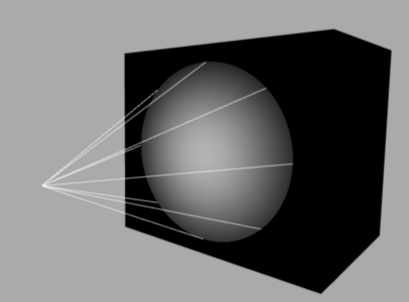
\includegraphics[width=1\linewidth]{images/chapter_baking_service/ba_se_ex_cubo.png}\hfill
 \caption[SpotLight ThreeJS]{Effetto di una SpotLight ThreeJS orientata verso un cubo.}
 \label{fig:ba_se_ex_cubo}
\end{figure}
Si consideri la spotlight in figura \ref{fig:ba_se_ex_cubo}:
per garantire un effetto più realistico è necessario agire su alcuni parametri, ad esempio diminuendo l’effetto luminoso in corrispondenza dei bordi del cono (exponent), e aumentando la dispersione della luce in funzione della distanza dalla superficie (decay). E’ necessario che la luce soddisfi queste proprietà, e che l’effetto complessivo sia confrontabile con quello delle luci che verranno create in blender.
\\ 
A questo punto vengono modellati i parametri di configurazione di ThreeJS con riferimento ai parametri di Blender che controllano gli stessi effetti. L’obiettivo è arrivare ad una condizione di equilibrio, trovando la configurazione di parametri ThreeJS, e di parametri Blender, avente come risultato due luci in due sistemi diversi, ma aventi effetti paragonabili.
\\
I parametri di Blender che controllano caratteristiche simili a quelle dei parametri decay ed exponent, sono il size e lo spot shape blend per le spotlight.
\\ 
Sperimentando configurazioni differenti e mettendo a confronto i risultati, si è arrivati ad un mappatura tipo tra i quattro parametri sopra citati, che consente un feedback visivo confrontabile tra SpotLight di ThreeJS e Spot Lamp di Blender.
\\
\begin{figure}[htb]
 \centering
 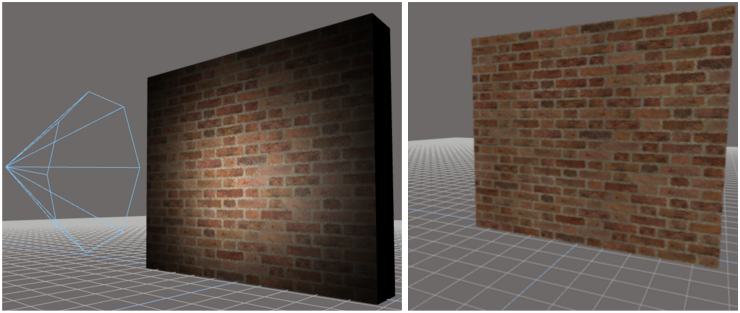
\includegraphics[width=1\linewidth]{images/chapter_baking_service/ba_se_confronto_spot.png}\hfill
 \caption[SpotLight preimpostata]{Effetto di una SpotLight ThreeJS preimpostata nell'editor (a sinistra), e risultato della replicazione della stessa nel bake (a destra).}
 \label{fig:ba_se_confronto_spot}
\end{figure}
A questo punto verrà descritta l’attività di mappatura con riferimento ai parametri di cui l’utente ha piena libertà di configurarne di valori nell’Editor, ovvero l’intensity, l’hex, e l’angle. Questi parametri non vengono preimpostati, e per ognuno di questi è possibile trovare un parametro corrispondente in Blender.
\\ 
Infatti vi sono delle nette corrispondenze tra spot shape size ed angle, intensity e strenght, hex e color. Gli effetti che intendono controllare questi parametri sono dunque gli stessi; ciò che cambia sono i valori che vengono assegnati a questi parametri.
\\
Questa situazione implica che nella fase di creazione delle luci, durante l’import della scena ThreeJS in Blender, per ogni luce venga letto dal JSON il valore di intensity e dato in input ad una funzione che, a partire da una valore di intensity interpretato da ThreeJS, restituisca un valore da assegnare al parametro Strenght per cui l’effetto di intensity della luce in ThreeJS venga replicato in Blender allo stesso modo. La procedura sarà la medesima per i parametri hex e angle.
\\ 
Il parametro intensity è quello che sicuramente ha richiesto più tempo per lo sviluppo di una funzione di mappatura, in quanto tale mappatura è diversa a seconda della luce che si sta utilizzando; ad esempio la sun Lamp di Blender, trovandosi infitamente lontana dall’origine della scena non utilizza per la strength la stessa unità di misura di una Spot o di una Point. La mappatura applicata è la seguente:
\\ 
All’interno dello script per importare la scena ThreeJS, se viene individuata la descrizione di un oggetto Light, viene invocata una funzione che si occupa esclusivamente di raccogliere la descrizione della luce, e generare in Blender una luce con le stesse caratteristiche. Durante la generazione per prima cosa viene individuato il tipo di luce; succesivamente, nel momento in cui viene individuata nel JSON la proprietà intensity della luce, se ne estrae il valore e in base al tipo di luce si mappa in un valore differente.
\begin{table}[]
\centering
\caption{Mappatura intensity Blender}
\label{insensity_table}
\begin{tabular}{|l|l|}
\hline
\textbf{Blender Lamp} & \textbf{Strenght Value} \\ \hline
Spot Lamp & intensity * 30000000 \\ \hline
Point Lamp & intensity * 500000 \\ \hline
Sun Lamp & intensity * 30 \\ \hline
\end{tabular}
\end{table}
Notare in tabella \ref{insensity_table} come per ogni luce il fattore di conversione sia differente; ogni fattore è studiato effettuando molteplici confronti tra gli effetti dell’intensity in ThreeJS con quelli della strenght in Blender. I risultati possono essere visti nella foto in figura \ref{fig:ba_se_tavolini}. 
\\
\begin{figure}[htb]
 \centering
 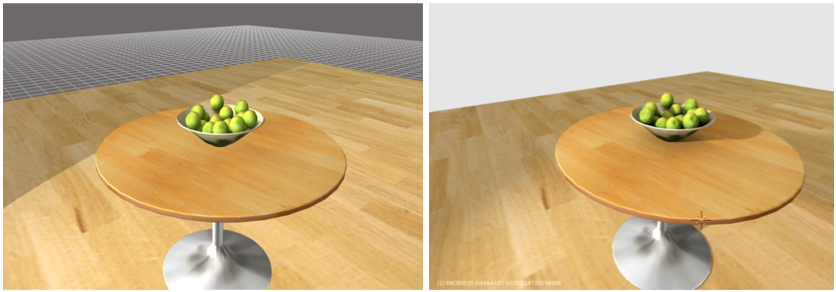
\includegraphics[width=1\linewidth]{images/chapter_baking_service/ba_se_tavolini.png}\hfill
 \caption[Confronto intensity - strenght]{Confronto tra illuminazione di una scena ThreeJS(a sinistra), e illuminazione della medesima scena importata in Blender (a destra).}
 \label{fig:ba_se_tavolini}
\end{figure}
Per quanto riguarda l’agle la mappatura è molto semplice, e riguarda esclusivamente la generazione di Spot Lamp.
\\
In presenza di un campo angle nella descrizione della luce nel JSON; il relativo valore viene estratto, moltiplicato per due, e assegnato al parametro spot shape size. 
\\
Infatti aggiungendo in ThreeJS e in Blender una spotlight con un valore angle uguale al valore spot shape size, la spot in Blender avrà un’angolo di apertura del cono che è la metà rispetto a quello di ThreeJS.
\\
L’ultimo parametro oggetto di mappatura è la componente RGB, ossia l’hex. Anche qui la situazione è semplice, in quanto la differenza è solo nella struttura dati con cui viene rappresentato il colore. Infatti mentre in ThreeJS il colore è rappresentato con un esadecimale a sei cifre, in Blender viene rappresentato con un vettore a quattro componenti, con valore compreso tra 0 e 1 (il quarto valore è l’Alpha, che nella descrizione JSON della luce è separato dell’informazione sul colore). 
\\
Anche in questo caso sarà la funzione dedicata alla generazione delle luci che si occuperà di individuare il parametro color nella descrizione JSON; in tal caso estrarrà dall’attributo l’esadecimale rappresentante il colore, e lo convertirà in un vettore mediante apposita funzione. 
\\
Per quanto riguarda le luci rimane da definire la mappatura per l’ambient light di ThreeJS.
Il colore di una Ambient Light viene applicato globalmente ad ogni elemento della scena, ed è uno strumento molto utile per avere ad esempio una base di illuminazione omogenea. L’ambient light così com’è intesa in ThreeJS non è presente come vera e propria Lamp all’interno di Blender, e pertanto ha richiesto uno stratagemma per essere replicata. Per effettuare questa operazione bisogna per prima cosa comprendere che l’unico parametro di configurazione di una Ambient Light è il suo colore. In Blender esiste un menu WORLD per la configurazione del mondo, ossia dell’intero ambiente 3D, e dell’illuminazione generale dello stesso. Questo menu contiene due parametri, \emph{color} e \emph{strenght} che determinano proprio il colore e la potenza con cui lo stesso viene irradiato in modo omogeneo su tutta la scena. Color e strenght saranno i parametri di Blender che verranno utilizzati per ricreare l’effetto di un’AmbientLight.
\\
Nel contesto del presente lavoro di tesi si fa l’assunzione che all’interno di una scena ThreeJS possa essere aggiunta un’unica AmbientLight. Questa conclusione nasce dal fatto che avere più ambient all’interno della scena comporterebbe solo una mescola dei colori che ognuna applica, ma la tonalità di tale mescola può comunque essere ottenuta aggiungendo un’unica ambient.
La funziona di mappatura consiste quindi nell’estrarre il colore dalla descrizione dell’ambient light nel JSON, e applicarlo al campo colore nel menù \emph{WORLD} di Blender.
\\
\begin{figure}[htb]
 \centering
 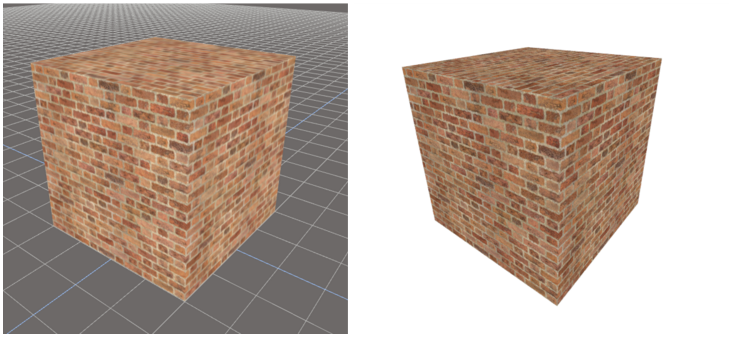
\includegraphics[width=1\linewidth]{images/chapter_baking_service/ba_se_confronto_cubi.png}\hfill
 \caption[Mappatura AmbientLight]{Confronto tra AmbientLight ThreeJS (a sinistra), e mappatura della medesima in Blender (a destra).}
 \label{fig:ba_se_confronto_cubi}
\end{figure}
E’ importante sottolineare che le operazioni di mappatura mostrate fin’ora sono strettamente correlate al tipo di motore di render utilizzato in Blender, ossia il Cycle Render. Basti pensare ad esempio che utilizzando il più leggero Blender Render, l’intensità delle luci in ThreeJS verrebbe mappata 1:1 con la strength delle rispettive luci in Blender. Anche per la distance si dovrebbe fare un discorso completamente diverso, perchè a differenza del Cycle Render, le SpotLight e le PointLight nel Blender Render hanno il parametro distance, che quindi può essere mappato direttamente da quello di ThreeJS.
\\
\\
La descrizione delle attività di mappatura esplicita dei parametri prosegue a questo punto con il mapping sui materiali.
In ThreeJS i materiali utilizzati più frequentemente sono il LambertMaterial per le superfici opache,e il PhongMaterial per le superfici brillanti.
Nel Cycles Render di Blender non ci sono veri e propri materiali, bensì dei \emph{surface shader} che regolano il modo in cui una luce viene riflessa dalla superficie di una mesh. Ogni shader è regolato da una funzione di distribuzione dibirezionale della dispersione \emph{(BSDF)}, ossia una funzione matematica che determina la probabiità che un raggio di luce venga riflesso con una certa angolatura. Nel Cycles Render di Blender ad ogni superficie può essere associato uno o più shader. Lo shader più utilizzato è sicuramente il Diffuse, la cui funzione di distribuzione è la medesima che regola il materiale Lambert. Da questo si può già evincere come il Lambert material di ThreeJS dovrà essere mappato in un surface shader di tipo Diffuse da applicare sulla superficie della mesh. 
\\
La mappatura avviene nel modo seguente: 
Come nal caso delle luci, gli input funzioni di mappatura saranno estratti dallo script di import che si impegna a riconoscere tutte le strutture descritte all’interno del JSON, e per ognuna invoca una funzione dedicata all’interpretazione della descrizione e alla generazione della rispettiva struttura Blender; in questo caso verrà mostrata la funzione che si prende carico di interpretare la descrizione di un materiale. Questa funzione è stata implementata sfruttando il \emph{node editor} di Blender, descritto nel paragrafago \ref{sec:chapter_tecnologie_abilitanti_blender}, le cui API sono molto semplici da utilizzare.
\\
La replicazione dei materiali in Blender avviene in modo diverso a seconda che la descrizione sia di un materiale Lambert o Phong. In entrambi i casi il risultato finale sarà comunque uno shader, che tramite il node editor verrà associato ad un nodo chiamato \emph{Material Output}. Questo nodo è un’astrazioe della superficie dell’oggetto; collegando uno shader a questo nodo equivale a mappare la funzione di distribuzione dello shader sulla superficie dell’oggetto.
\\
Indipendentemente dal tipo di materiale, per prima cosa vengono estratte due informazioni dalla descrizione, ovvero l’\emph{alpha} e il \emph{colore}, quest’ultimo convertito sempre nello stesso formato utilizzato per le luci. 
\\
Dopodichè viene istanziato nel node editor uno shader \emph{Diffuse BSDF}, indipendentemente dal tipo di materiale che si sta interpretando; verrà mostrato infatti come la mappatura del Phong non avrà un vero e proprio shader Phong corrispondente, ma un mix tra glossy shader e diffuse shader.
A questo punto il processo di mappatura differisce a seconda del tipo di materiale da replicare. Il primo processo che verrà descritto riguarda la mappatura del materiale Lambert.
Un nodo Diffuse BSDF ha degli input e un’output, che è la funzione di riflessione da applicare alla superficie.
\\
Tra gli input ci sono il colore della superficie, la rugosità della stessa, e le normali. Il colore della superficie corrisponde a quello estratto dalla descrizione, e al vettore R,G,B corrispondente viene aggiunto l’alpha estratto sempre allo stesso modo.
\\
Se nel materiale non e presente la descrizione di alcuna texture, è sufficiente associare lo shader Diffuse alla superficie della mesh, che quindi godrà di una riflessione lambertiana sulla lunghezza d’onda del colore impostato. 
\\
\begin{figure}[htb]
 \centering
 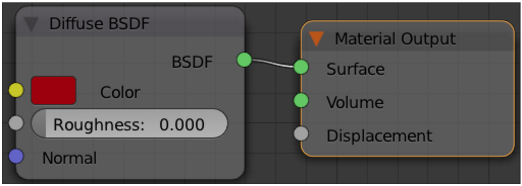
\includegraphics[width=1\linewidth]{images/chapter_baking_service/ba_se_diffuse.png}\hfill
 \caption[Diffuse shader Blender]{Esempio di nodo Diffuse Shader collegato al Material Output.}
 \label{fig:ba_se_diffuse}
\end{figure}
La texturizzazione verrà mostrata più avanti, in quanto risulta invariata sia per un lambert che per un Phong.
\\ 
Per quanto riguarda la mappatura del materiale Phong, si è già menzionato il fatto che il questo tipo di materiale viene utilizzato quando si trattano superfici brillanti. Pertanto la replicazione in Blender del materiale Phong viene fatta solo se il valore di brillantezza del materiale, o \emph{shininess}, è sufficientemente alto (oltre i 30 punti); in caso contrario un valore basso di shininess porterebbe ad un feedback visivo del materiale molto simile a quello del Lambert, e quindi verrebbe importato come tale. 
\\
Per la replicazione di un materiale Phong viene creato uno shader di tipo glossy da associare a quello diffuse gia creato. Il \emph{glossy shader} viene usato per le riflessioni lucide, specialmente in materiali metallici o specchi. Anche questo shader avrà come output la funzione BSDF da associare alla superficie della mesh, mentre in input prenderà il colore della superficie, un parametro \emph{roughness} che influenza la nitidezza della riflessione, e un parametro \emph{Distribution}, che indica il tipo di riflessione (ad es. perfettamente nitida con \emph{Sharp}, o influenzata dalla roughness con \emph{Beckmann}). Per un mapping del materiale Phong verrà utilizzata la distribuzione Beckmann; questo perchè il fattore di riflessione deve poter variare a seconda di come l’utente ha impostato la shininess in ThreeJS. I parametri shininess di ThreeJS e roughness di Blender sono tuttavia rappresentati in formati completamente diversi: mentre la roghness è un valore di ruvidezza, e quindi più è alto più la superficie è opaca, la shininess è un valore di brillantezza, e quindi più è alto più la superficie è lucida. Inoltre mentre la shininess è rappresentata da un intero compreso tra 1 e 500, la roughness è un valore compreso tra 0 e 1, estremi inclusi.
\\
E’ evidente dunque la necessità realizzare una funzione di mappatura dello shininess ThreeJS in un valore di roughness Blender. A tale scopo è stato effettuato uno studio di funzione per capire quale potesse essere l’equazione di una funzione per la regolazione della roughness al variare della shininess. Per calcolare l’equazione, sono stati individuati in uno spazio 2D un buon numero di punti $(x,y)$ dove la x corrisponde alla roughness e la y alla shininess. Per fissare un punto nello spazio è stato attuato un confronto visivo tra materiale Phong replicato in Blender e Phong di ThreeJS. Se, per una determinata mesh, il valore di roughness $r$ in Blender e il valore di shininess $s$ in ThreeJS portavano ad un feedback visivo di brillantezza del materiale paragonabile tra i due sistemi, allora il punto $(s,r)$ veniva individuato nello spazio 2D. 
\\
\begin{figure}[htb]
 \centering
 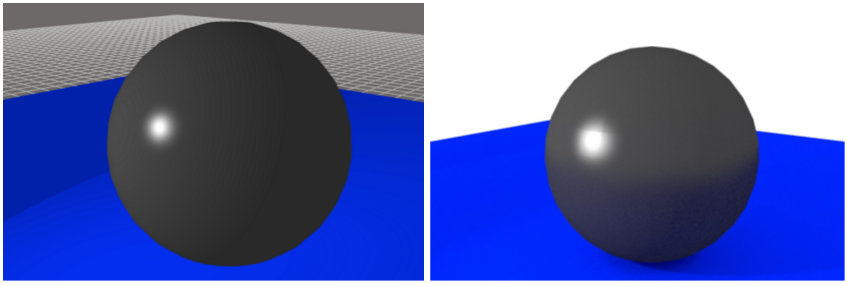
\includegraphics[width=1\linewidth]{images/chapter_baking_service/ba_se_sferephong.png}\hfill
 \caption[Mapping Phong material]{Confronto tra una sfera con material Phong ThreeJS (a sinistra), e medesima sfera importata in Blender (a destra).}
 \label{fig:ba_se_sferephong}
\end{figure}
Posizionati nello spazio un certo numero di punti, si è individuata la funzione passante per tutti i punti definiti, o comunque una buona approssimazione di questa. 
\\
La differenza tra gli intervalli numerici dei due parametri non ha permesso tuttavia  l’individuazione di un’unica funzione che mappasse fedelmente la roughness dato un valore qualsiasi all’interno dell’intero range di valori di shininess. 
\\
Nonostante la funzione fosse calcolabile, testando il mapping sull’intero range di valori di entrambi i parametri i risultati di roughness, a fronte di quelli di shininess, non erano paragonabili dal punto di vista del feedback visivo. La soluzione è stata dunque quella di spezzare gli intervalli di entrambi i parametri e per ogni porzione definire una funzione di mappatura differente. 
\\
Una volta individuata sia la distribuzione che il valore di roughness da assegnare al glossy shader, il passo successivo prevede di impostare il colore del glossy shader su tonalità scure, in modo da riflettere solo la luce e non l’ambiente circostante.
Si ricorre a questo stratagemma perchè il glossy shader viene utilizzato per le superfici riflettenti, ma nel presente contesto applicativo è necessaria solamente la brillantezza data dal riflesso della luce, e non la riflessione dell’ambiente circostante. 
Una volta impostata la parte dello shader che si occupa dell’effetto brillantezza del phong, bisogna creare lo shader che imposta il colore diffuse sulla superficie, che provenga da una texture o da una semplice componente RGB.
\\
A tale scopo viene si utilizza lo shader diffuse creato in precedenza. Ciò che viene configurato di questo shader è solamente il colore, e possono esserci due casi possibili:
Se al materiale non deve essere associata alcuna texture, il colore del diffuse sarà quello estratto dalla descrizione del materiale, esattamente come nel caso Lambert senza texture; se invece la superficie deve essere texturizzata, allora il colore dello shader diffuse viene impostato a nero. Questa procedura è fondamentale perchè il contributo del colore diffuse della texture non deve essere alterato in alcun modo da altre fonti, e impostando il colore dello shader a nero equivale a sommare all’RGB diffuse della texture una componente RGB composta da $(0,0,0)$, mantenendo dunque invariato il risultato. 
\\
Infine vengono combinati gli effetti dello shader diffuse e glossy in un unico shader, e la rispettiva funzione BSDF viene mappata sulla superficie della mesh. 
E’ importante sottolineare il fatto che in Blender viene mappato un materiale Lambert anche se il materiale descritto nel JSON è di tipo Basic. La proprietà Basic di non dipendere da alcuna fonte luminosa viene rispettata mediante configurazione lato client di un parametro realizzato appositamente per lo scopo.
\\
L’ultima fase nel processo di mappatura di un materiale in Blender riguarda la texturizzazione.
Questo processo è il medesimo sia per l’import di materiali con riflessione Lambertiana che per materiali Phong; l’unica differenza è nella combinazione degli shader finali. 
\\
Il processo di texturizzazione ha inizio nel momento in cui la funzione di import dei materiali in Blender, implementata nello script bake.py discusso nel paragrafo \ref{sec:chapter_baking_service_pipeline_baking_caricamento_scena}, dopo aver replicato il materiale descritto nel JSON individua nella medesima descrizione un parametro “map”. Questo parametro implica l’esistenza di una descrizione di texture all’interno del materiale, che deve essere quindi interpretata per texturizzare la superficie della mesh. Il compito di interpretare la descrizione della texture nel JSON, e di texturizzare la superficie della mesh, è a carico di un’apposita funzione. I passi svolti da questa funzione sono i seguenti: 
Dopo l’estrazione del base64 della texture dalla descrizione JSON, e la decodifica nella corrispondente immagine, viene istanziato un nodo di tipo Image Texture. Questo nodo rappresenta il blocco dati dell’immagine; siccome ogni texel di un’immagine è caratterizzato da una componente di colore RGB, l’output di un nodo di questo tipo può essere inteso come colore RGB dell’immagine. Questo colore può quindi essere dato in input ad uno shader diffuse, che si occuperà di mappare tale colore sulla superficie della mesh. 
\\
\begin{figure}[htb]
 \centering
 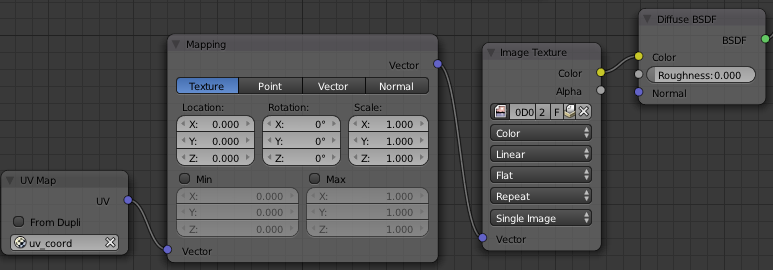
\includegraphics[width=1\linewidth]{images/chapter_baking_service/ba_se_diffuse_uv_ma.png}\hfill
 \caption[Mappatura texturizzazione]{In foto è mostrato un dettaglio circa la configurazione di nodi che permette di applicare una texture ad un oggetto.}
 \label{fig:ba_se_diffuse_uv_ma}
\end{figure}
Nel paragrafo \ref{sec:chapter_stato_arte_lightmap} si è discusso di come la condizione abilitante per un corretto mapping di una texture su di una superficie sia l’utilizzo delle mappe UV. Questa procedura viene svolta generando un nodo UV Map rappresentante proprio la mappa UV, e assegnando a questo nodo i valori della mappa UV estratta dalla descrizione della texture nel JSON. Questo nodo viene poi collegato al nodo Texture, come è mostrato in figura \ref{fig:ba_se_diffuse_uv_ma}
\\
L’attività di texturizzazione deve inoltre tenere conto di alcuni parametri configurabili all’interno dell’editor. 
\\
Durante un’utilizzo tipico dell’editor da parte dell’utente, può essere necessario ripetere più volte la texture sulla superficie, ad esempio quando nella realizzazione di un pavimento si vuole replicare un motivo su tutta la superficie. Il fattore di replicazione di una texture sui due assi $x$ e $y$ viene inserito all’interno della descrizione JSON della texture.
\\
Similmente a quanto visto per la roughness del glossy shader in Blender, e la shininess del PhongMaterial in ThreeJS, ci sono differenze nel formato tra repeat in ThreeJS e repeat nel Cycle Render di Blender.
\\
In ThreeJS il repeat è descritto mediante un vettore con due valori $x$ e $y$; $x$ è un intero che indica il numero di volte che la texture deve essere replicata lungo l’asse $x$; la $y$ indica invece il numero di ripetizioni sull’asse $y$. Il processo di ripetizione consiste nel suddividere la superficie lungo l’asse $x$ e $y$ un numero di volte indicato dal fattore repeat; si ottiene così una superficie suddivisa in più sezioni. A questo punto la texture viene applicata su ogni sezione ottenendo quindi l’effetto di ripetizione della stessa.
\\
Nel Cycle render di Blender il repeat viene applicato in modo simile, ma per farlo  bisogna intervenire sulle UV Map. E’ necessario infatti definire un fattore di scalatura lungo gli assi $u$ e $v$, della UV Map. Se 1 è la scala originale della UV Map, un fattore di scalatura 0.5 sull’asse $u$ implica che lungo tale asse la mappa sarà grande la metà dell’originale, e quindi su tale asse può essere replicata; lo stesso vale per l’asse $v$. Siccome la mappa UV viene replicata, la texture verrà mappata sulla superficie in corrispondenza di ogni replica, ottenendo quindi l’effetto ripetizione. Da questa descrizione si può notare sin da subito come la rappresentazione numerica del repeat nei due sistemi sia una l’opposto dell’altra. In ThreeJS sono due interi maggiori di 0 che indicano esplicitamente il numero di ripetizioni lungo i due assi di riferimento, in Blender sono due valori compresi tra 0 e 1 che indicano la percentuale di scalatura della mappa UV rispetto agli assi di riferimento. Siccome i valori sono uno l’inverso dell’altro, è possibile definire una mappatura del repeat in Blender calcolando l’inverso dei due valori di repeat per $x$ e $y$ descritti per la texture nel JSON. Questa mappatura è implementata all’interno della funzione che si occupa di importare le texture in Blender. Siccome il repeat si applica sulla mappa UV, bisognerà intervenire sul nodo del node editor che la rappresenta. L’intervento consiste nell’inserimento tra il nodo Texture e il Nodo UV Map di un nodo intermedio detto \emph{Mapping}, mostrato in figura \ref{fig:ba_se_diffuse_uv_ma} . Questo nodo intermedio si occupa di prendere in input la mappa UV e applicare su di essa una scalatura sugli assi $x$ e $y$, che corrispondono agli assi $u,v$ trattandosi di una UV map. L’output di questo nodo sarà la mappa UV ripetuta, che verrà quindi data in input al nodo Texture. I fattori di scaling da inserire nel nodo Mapping sono calcolati dalla funzione di import delle texture, che estrae i repeat $x$ e $y$ ThreeJS della descrizione JSON della texture e che al parametro di scaling sulle u del nodo Mapping assegnerà il valore $\frac{1}{x}$, mentre al parametro di scaling sulle $v$ assegnerà $\frac{1}{y}$.
\\
A questo punto si è ottenuto un nuovo shader diffuse per il mapping della texture sulla superficie della mesh. L’ultima fase prevista dalla texturizzazione è la combinazione di questo nuovo shader, con quello del materiale già realizzato. La combinazione è possibile utilizzando un nodo \emph{Mixer}, che prende in input i due shader e ne produce uno unico da assegnare alla superficie della mesh. Come già menzionato in precedenza è importante che, per una texturizzazione fedele dei diffuse color dell’immagine, gli eventuali contributi di colore di altri shader vengano impostati sul nero, in modo da non influenzare il colore della texture. Per questo motivo prima della texturizzazione vengono controllati gli shader, ed eventuali contributi di colore vengono impostati a nero $(0,0,0)$. 